\chapter*{Introduction} 
\addcontentsline{toc}{chapter}{Introduction}

\section{Objectives}
\section{Acomplishments}

% The first ever game created was 'Tennis for Two' and was played on an oscilloscope. From then, gaming evolved from simple pixelated experiences to complex, immersive digital worlds.

% "Before game engines, games were typically written as singular entities: a game for the Atari 2600, for example, had to be designed from the bottom up to make optimal use of the display hardware (...) 
% Even on more accommodating platforms, very little could be reused between games."

% (Game Engine, Wikipedia)

% % (Did u know that the first Roller Coaster Tycoon was written completly in Assembly?)

% Programmers needed a way to make the game building process more efficient. So around the mid-1990s, thanks to Epic Games and their launch of the Unreal Engine and thanks to Id Software's Doom and Quake games the term "Game Engine" started to become more and more popular.

% Fast forward mid-2020s, now we have access to ultra realistic tank simulators for soldier training ( projectName ), surreal worlds filled with fantasy creatures ( Middle Earth: Shadow Of Mordor ) and even indie projects like Hyerbolica that portraits how a non-euclidian world would behave like. Projects like these would've been way harder ( if not actually impossible ) to pull off without the help of game engines.

% \pagebreak

% \section{Game Engines}
% "The line between a game and its engine is often blurry. Some engines make a reasonably clear distinction, while others make almost no attempt to separate the two. ( ... ) We should probably reserve the term
% 'game engine' for software that is extensible and can be used as the foundation for many different games without major modification."

% ( Game Engine Architecture. by Jason Gregory )

% \begin{figure}[!h]
%     \centering
%     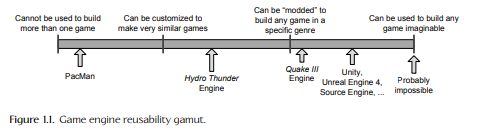
\includegraphics[width=1\linewidth]{chapters/gameEngine Usability.png}
%     \caption{Game Engine Reusability Gamut}
%     \label{fig:Game-Engine Reusability}
% \end{figure}



% Behind the curtains of any interactive application there is most likely a Game Engine. 
% You have probably heard before about Unity and Unreal but there are many more game engines out there. Some of them are In-House, some of them are Open-Source, some of them are made for a specific Genre. But none of them is offering Built-In Machine Learning Integration. 

% \subsection{What does a Game Engine offer?}

% While not limited to, some of the tools we expect a game engine to offer are: 
% \begin{enumerate}
%     \item Input Handling
%     \item Player Mechanics
%     \item Game-Specific Rendering
%     \item Collision \& Physics
%     \item Audio Playback
%     \item Game Cameras
%     \item Ai \& Behaviour Management
%     \item Online Multiplayer
%     \item Scene Graph
%     \item Scripting System
%     \item Visual Effects
% \end{enumerate}

% \section{What is Machine Learning?}

% \begin{enumerate}
%     \item predicts text, predicts what the next word in a sentence would most likely be.
%     \item it's too broad of a topic to be able to explain in detail in just one paper. And it's also not the purpose of this paper. This paper only wants to use the power of ai to simulate better npc's in games.
%     \item for the purpose of this, i will not try to recreate or train an machine learning model, i will use an already existing one: GPT 3.5-Turbo by OpenAI.
% \end{enumerate}

% \subsection{Machine Learning in Game Engines}
% \begin{enumerate}
%     \item Inworld Origins are already working on a solution for implementing GPT4 to be used in a NPC dialogue scenario.
%     \item There is this study where multiple GPT4 agents that can simulate believable human behavior. (Generative Agents: Interactive Simulacra of Human Behavior)
%     % https://arxiv.org/pdf/2304.03442.pdf
%     \item Currently, there are no game engines that have Machine Learning Systems built-in. 
% \end{enumerate}

% \section{Scope and Objectives of the Thesis}
% \begin{enumerate}
%     \item exploration, development, and evaluation of a game engine that integrates GPT-based machine learning capabilities 
%     \item explore the architecture of a game engine while building a basic one in Python using OpenGL.
%     \item explore what it means to add machine learning capabilities to a game engine. 
%     \item The focus of this research is on leveraging the power of natural language processing (NLP) and GPT models to enhance various aspects of game development, including storytelling, character interactions, procedural content generation, and player experiences.
% \end{enumerate}

